%!TEX root = main.tex
\section{Pose Detection}


\begin{frame}
\frametitle{Problem Definition}

\begin{itemize}
\item A pose is the temporary suspension of the animation of the body joints in a discrete configuration.
\item Pose detection is the problem of automatically classifying a pose.
\item \textit{Poses can be used as control signals}
\end{itemize}
\end{frame}


\begin{frame}
\frametitle{Assumptions}

\begin{itemize}
\item Sufficient room \textbf{lighting} conditions for the operation of the Kinect sensor
\item User is positioned \textbf{inside the operating area} of the Kinect sensor and is \textbf{facing} the sensor
\item \textbf{Predefined} set of target poses
\end{itemize}

\end{frame}

\begin{frame}
\frametitle{Design Prerequisites}

Detection is

\begin{itemize}
\item \textbf{real-time}
\item invariant to the user \textbf{position} and \textbf{distance} from the camera
\item invariant to the user \textbf{physical characteristics} (height, weight etc.)
\item able to support \textbf{multiple users} (a limit of 2 is imposed by the Kinect sensor)
\end{itemize}

\end{frame}

\begin{frame}
\frametitle{The proposed algorithm}

\begin{itemize}
\item Template matching to a set of geometric features
\item Poses are predefined templates
\item We compare the current feature vector to the template, and if it is within a predefined error margin the pose is recognized
\end{itemize}

\begin{center}
\textbf{Simple, fast and performs well in real world scenarios.}
\end{center}

\end{frame}

% %!TEX root = main.tex
\subsection{The Microsoft Kinect SDK}


\begin{frame}
\frametitle{Data streams}

\begin{figure*}[ht!]
  \centering
  \begin{minipage}{0.32\textwidth}
  	\centering
    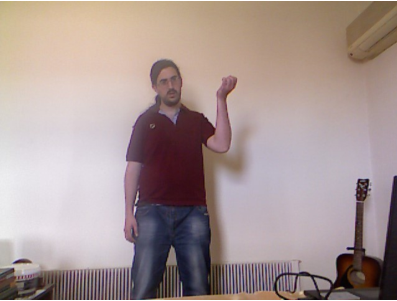
\includegraphics[width=\textwidth]{figs/color-frame}\\
    Color Stream
  \end{minipage}\hfill
  \begin{minipage}{0.32\textwidth}
  	\centering
	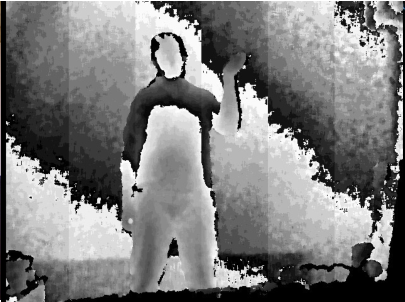
\includegraphics[width=\textwidth]{figs/depth-frame}\\
    Depth Stream
  \end{minipage}\hfill
  \begin{minipage}{0.32\textwidth}
  	\centering
    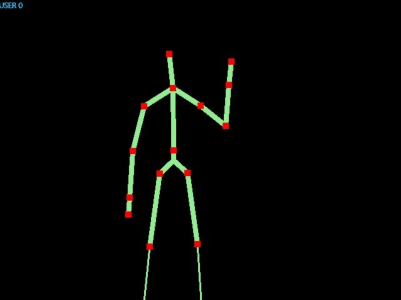
\includegraphics[width=\textwidth]{figs/skeleton-frame}\\
    Skeleton Stream
  \end{minipage}
\end{figure*}

\end{frame}


\begin{frame}
\frametitle{Skeleton Joints}
\begin{itemize}
\item A total of 20 inferred joints
\item Organized in a hierarchical structure (we make use of this later)
\end{itemize}

\begin{figure*}[ht!]
\label{fig1}
\centering
\begin{minipage}{0.34\linewidth}
\centering
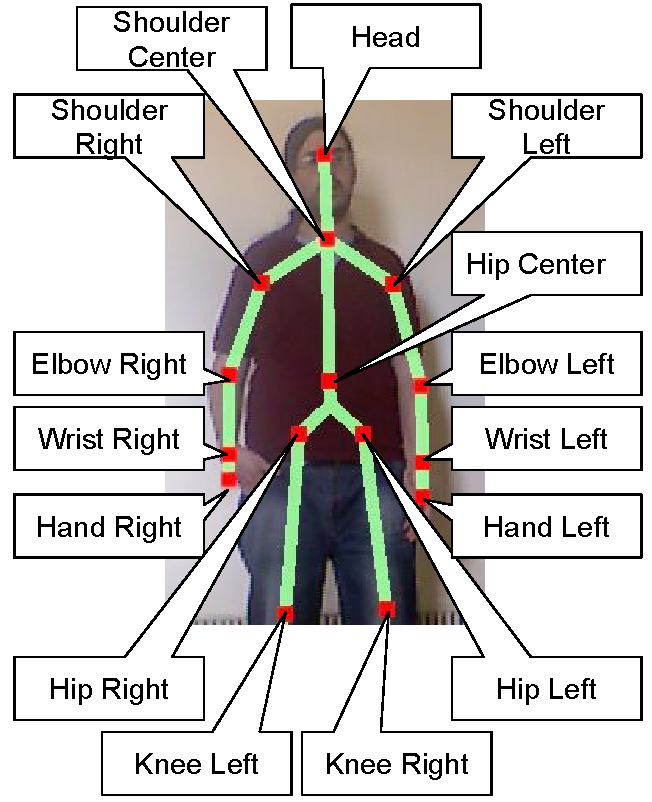
\includegraphics[width=\linewidth]{figs/skeleton.pdf}\\
Skeletal Joints
\end{minipage}\hfill
\begin{minipage}{0.6\linewidth}
\centering
\resizebox{\linewidth}{!} {
\tikzset{edge from parent/.style=
{draw, edge from parent path={(\tikzparentnode.south)
-- +(0,-3pt)
-| (\tikzchildnode)}},
blank/.style={draw=none}}
    \begin{tikzpicture}

    \node{\Tree 
     [.{HipCenter} 
        [.Spine [.{Shoulder Center}  [.{Shoulder Left} [.{Elbow Left} [.{Wrist Left} [.{Hand Left} ]]]]  {Head} [.{Shoulder Right} [.{Elbow Right} [.{Wrist Right} [.{Hand Right} ]]]]  ]]
        [.{Hip Left} [.{Knee Left} [.{Ankle Left} [.{Foot Left} ]]]]
        [.{Hip Right} [.{Knee Right} [.{Ankle Right} [.{Foo tRight} ]]]]
        ]};
    \end{tikzpicture}
}\\
Joints in a tree structure
\end{minipage}

\end{figure*}
\end{frame}


\subsection{The Algorithm}

\begin{frame}
\frametitle{Geometric Features}

\begin{itemize}
\item Make use of the joints \textbf{hierarchical} structure to compute the \textbf{angles between} each \textbf{parent} and \textbf{child} joint.

\item This \textbf{single} feature provides by default the \textbf{position} and \textbf{depth invariance} and is \textbf{enough} to classify a \textbf{large set} of poses.
\end{itemize}
\end{frame}

\begin{frame}
\frametitle{Feature Calculation}


\begin{figure}[!htb]
\centering
\resizebox{0.3\linewidth}{!} {
  \begin{tikzpicture}[scale=1]
     \coordinate (A) at (2,5);
     \coordinate (B) at (6,3); 
     \coordinate (C) at (2,0);
     \draw (A) -- (B) node [anchor=south]{$B$} node [midway, above] {$c$};
     \draw (B) -- (C) node [anchor=north]{$C$} node [midway, right] {$a$};
     \draw (C) -- (A) node [anchor=south]{$A$} node [midway, left] {$b$};
     \tkzMarkAngle(B,C,A);
   \end{tikzpicture}
}\\
\small The triangle that is formed between the father joint $A$, the child joint $B$ and the point $(A.x, 0)$
 \end{figure}

Using the law of cosines, we calculate the $\angle{ACB}$ as

\begin{equation}
C=\cos^{-1}\frac{a^2+b^2-c^2}{2ab}
\end{equation}

\end{frame}

\begin{frame}[fragile]
\frametitle{Example Pose Template}

\begin{columns}[T]
\begin{column}{.5\linewidth}

\begin{figure}[!ht]
\centering
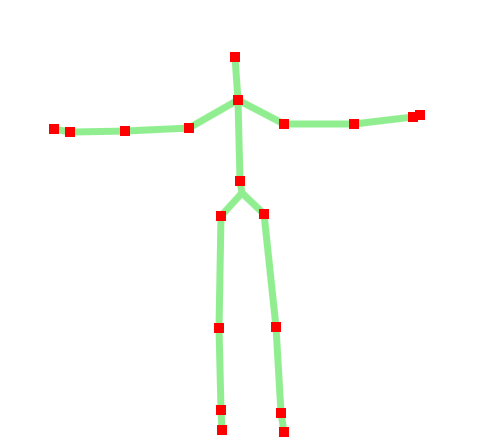
\includegraphics[width=\linewidth]{figs/hands-apart-pose.png}
\end{figure}

\end{column}

\pause

\begin{column}{.5\linewidth}

\begin{minipage}{\linewidth}

\lstset{
   basicstyle=\ttfamily,
   columns=fullflexible,
   showstringspaces=false%,
%   commentstyle=\color{gray}\upshape
 }

\begin{lstlisting}[
    basicstyle=\tiny, %or \small or \footnotesize etc.
]
 <?xml version="1.0" encoding="utf-8" ?>
 <Pose id="HANDSAPART"
       xmlns:xsi="http://www.w3.org/2001/XMLSchema-instance"
       xsi:schemaLocation="urn:PoseRules PoseRules.xsd">
     <DisplayName>Jack I'm Flying</DisplayName>
     <AngleConstraints units="degrees">
         <ElbowLeft>
             <Desired>180</Desired>
             <Deviation>15</Deviation>
         </ElbowLeft>
         <HandLeft>
             <Desired>180</Desired>
             <Deviation>15</Deviation>
         </HandLeft>
         <ElbowRight>
             <Desired>0</Desired>
             <Deviation>15</Deviation>
         </ElbowRight>
         <HandRight>
             <Desired>0</Desired>
             <Deviation>15</Deviation>
         </HandRight>
     </AngleConstraints>
 </Pose>
 \end{lstlisting}
\end{minipage}
\end{column}

\end{columns}

\end{frame}
